\section{Morfologisk analyse af mekaniske dele} \label{Morfologisk analyse - mekaniske dele}
Alle delfunktioner, der omhandler mekaniske dele beskrevet i afsnit \ref{Funktioner}, opsættes i en morfologisk analyse, hvor delløsninger til hver enkelt delfunktion benyttes til at danne samlede løsningskoncepter. Koncepterne skal overholde alle de ufravigelige krav opsat i afsnit \ref{Endelige kravspecifikationer}, for at blive medtaget i den morfologiske analyse.

Antallet af kombinationer af delløsninger, er vurderet for stor til at alle koncepter har kunne gennemgås. Der er fravalgt delløsninger, på baggrund af mangel på effektivitet og nøjagtighed. Der er udvalgt ni koncepter der arbejdes videre med, disse koncepter kan ses i tabel \ref{tab: morfologisk analyse af mekanikse}. Konceptforslagene fra den morfologiske analyse, kan findes ved at følge de forskellige farver/former, der hver repræsenterer et koncept skabt af delkoncepter.


%en farve/form hvert element i det bestemte koncept. Ved at følge for eksempel den lilla cirkel ($\lillacirc$), findes alle delkoncepterne som koncept 1 består af.

%Antallet af kombinationer af delløsninger, har resulteret i en mængde af koncepter vurderet for stor til at alle koncepter har kunne gennemgås

\begin{table}[H]
   \caption{Morfologisk analyse. 1 $=$ \protect\lillacirc, 2 $=$ \protect\bluebox, 3 $=$ \protect\cyanbox, 4 $=$ \protect\blueangle, 5 $=$ \protect\greenangle, 6 $=$ \protect\gulangle, 7 $=$ \protect\orangeangle, 8 $=$ \protect\pinkstar og 9 $=$ \protect\redkant}
    \centering
    \begin{tabular}{|l|p{3.1cm}|p{3.1cm}|p{3.1cm}|p{3.1cm}|} \cline{2-5}      
           \multicolumn{1}{l|}{} & \multicolumn{4}{|c|}{\cellcolor{aaublue} \textcolor{white}{\textbf{Delkoncepter til mekaniske delfunktioner }}} \\ \cline{2-5} \multicolumn{1}{l|}{}  & \multicolumn{1}{c|}{ \cellcolor{lightgray!20} \textbf{1}} & \multicolumn{1}{|c|}{\cellcolor{lightgray!20} \textbf{2}} & \multicolumn{1}{c|}{\cellcolor{lightgray!20} \textbf{3}} & \multicolumn{1}{c|}{\cellcolor{lightgray!20} \textbf{4}}  \\ \cline{2-5} \specialrule{0pt}{0.5pt}{0pt}
          
        %Bevægelse
        \rotatebox[origin=c]{90}{\cellcolor{aaublue} \textcolor{white}{\textbf{Bevægelse }}} & \makecell{\small Lineær bevægelse  \\ \includegraphics[width=0.98\linewidth]{Sections/5 Konceptgenerering/Media/lineær.png} \\ \lillacirc \ \bluebox \ \orangeangle \ \redkant} & \makecell{\small Robotarm \\ 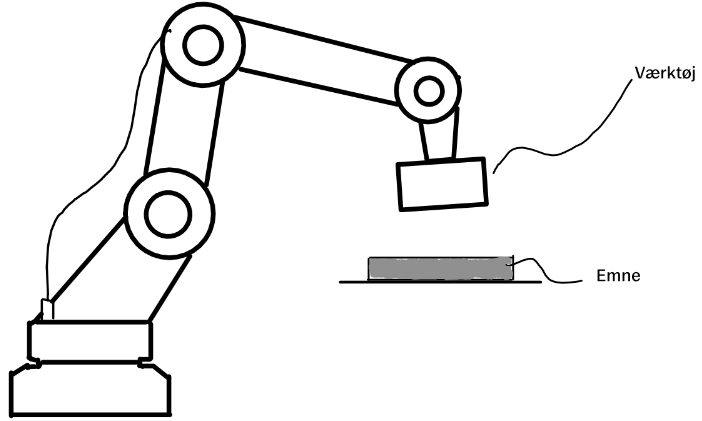
\includegraphics[width=0.98\linewidth]{Sections/5 Konceptgenerering/Media/arm.png} \\ \gulangle} & \makecell{\small Deltarobot\\ 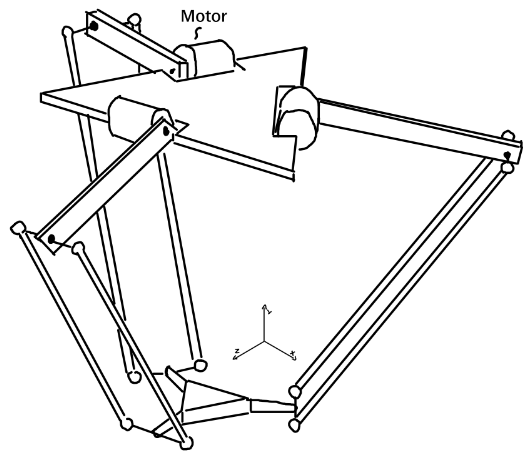
\includegraphics[width=0.98\linewidth]{Sections/5 Konceptgenerering/Media/delta.png} \\ \cyanbox \ \blueangle \ \pinkstar } & \makecell{\small Drejeskive \\ 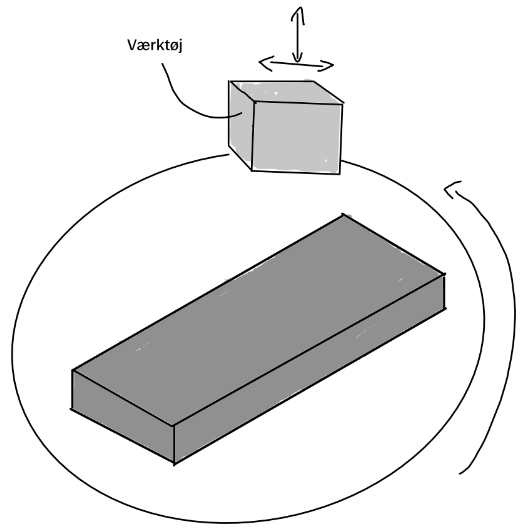
\includegraphics[width=0.98\linewidth]{Sections/5 Konceptgenerering/Media/Drejeskive.png} \\ \greenangle}\\  \specialrule{1pt}{0pt}{0pt}


        %Sæt prik
        \rotatebox[origin=c]{90}{\cellcolor{aaublue} \textcolor{white}{\textbf{\small Sætte prikker}}} & \makecell{\small Sætte dråbe \\ \includegraphics[width=0.8\linewidth]{Sections/5 Konceptgenerering/Media/åbnelukke.png} \\ \lillacirc \ \bluebox \ \cyanbox \ \blueangle \ \greenangle }& \makecell{ \small Spids røre  \\ emnet \\ \includegraphics[width=0.2\linewidth]{Sections/5 Konceptgenerering/Media/spids røre.png} \\ \gulangle \ \orangeangle \ \pinkstar \ \redkant} & \makecell{\small Spray \\ 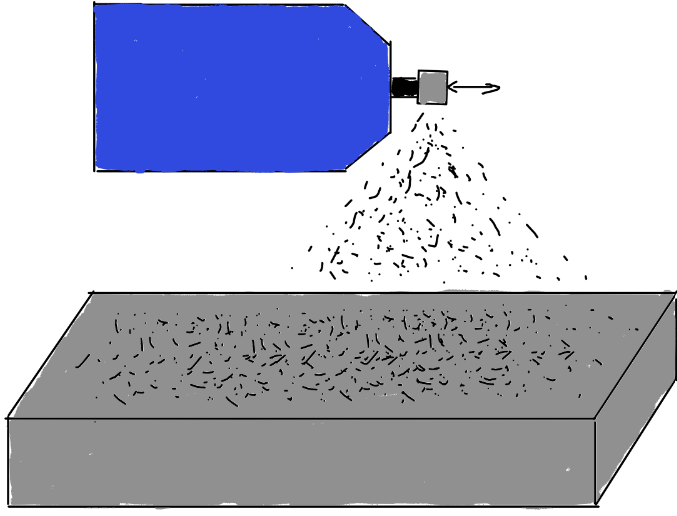
\includegraphics[width=0.8\linewidth]{Sections/5 Konceptgenerering/Media/spray.png}} & \makecell{\small Stempel \\ 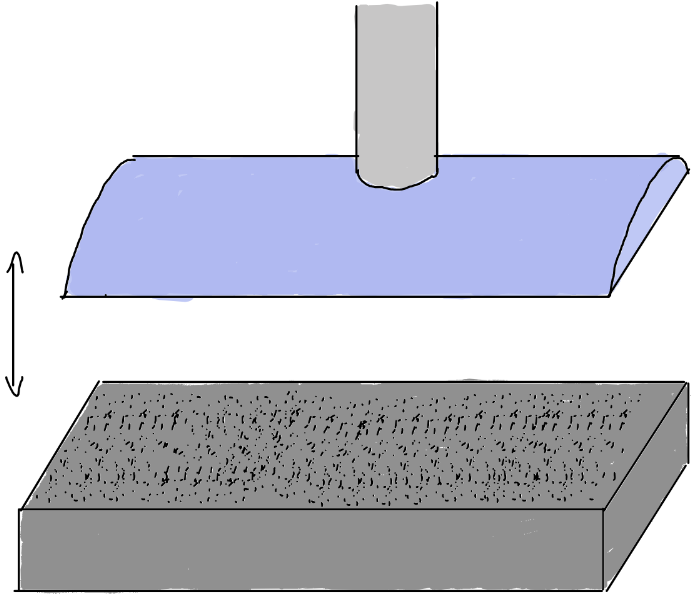
\includegraphics[width=0.98\linewidth]{Sections/5 Konceptgenerering/Media/stempel.png}}  \\ \specialrule{1pt}{0pt}{0pt}

        %Indspænding
        \rotatebox[origin=c]{90}{\cellcolor{aaublue} \textcolor{white}{\textbf{Indspænding}}} & \makecell{\small Press på emnet \\ \includegraphics[width=0.7\linewidth]{Sections/5 Konceptgenerering/Media/Press på emnet.png} \\ \bluebox \ \orangeangle \ \gulangle}  & \makecell{Sug \\ 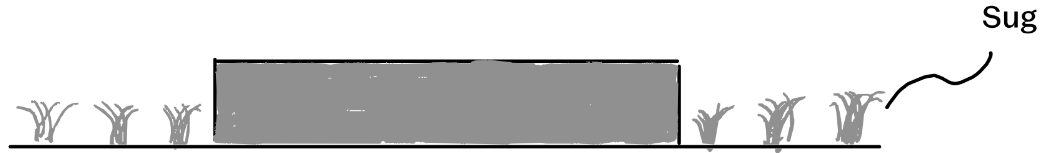
\includegraphics[width=0.98\linewidth]{Sections/5 Konceptgenerering/Media/sug.png} \\ \lillacirc \ \redkant} & \makecell{\small Vakuumpose\\ med fyld \\ 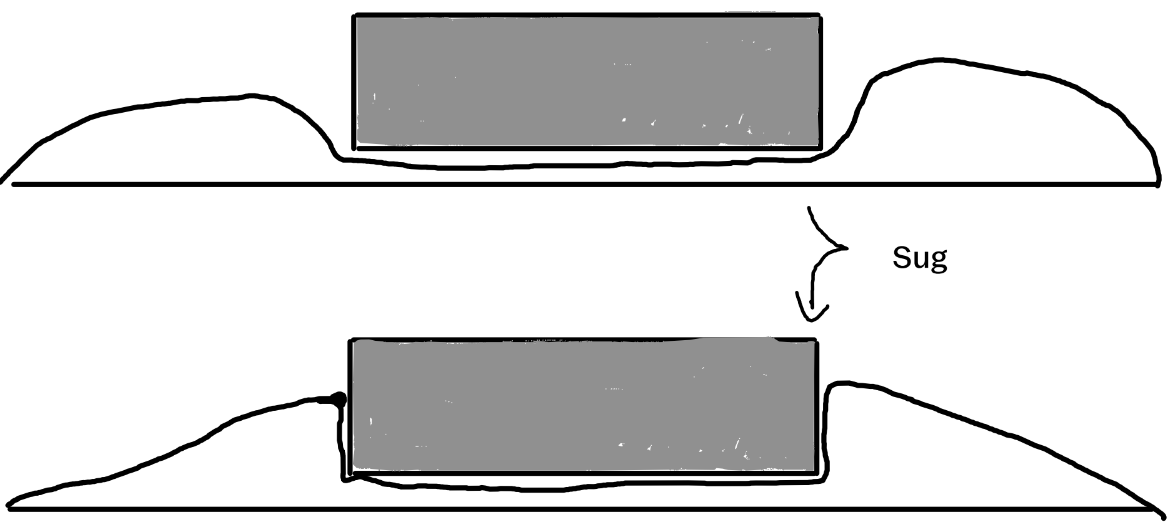
\includegraphics[width=0.98\linewidth]{Sections/5 Konceptgenerering/Media/vakuum.png} \\ \cyanbox \ \greenangle \ \pinkstar}&  \makecell{\small Ru overflade \\ 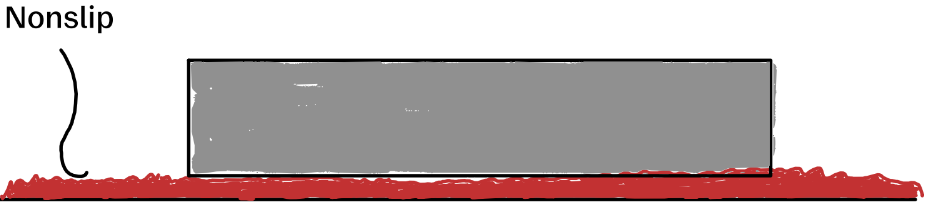
\includegraphics[width=0.98\linewidth]{Sections/5 Konceptgenerering/Media/rug.png} \\ \blueangle}  \\ \specialrule{1pt}{0pt}{0pt}

        %Understøttelse
        \rotatebox[origin=c]{90}{\cellcolor{aaublue} \textcolor{white}{\textbf{Understøttelse}}} & \makecell{\small Plade \\ under emnet \\ \includegraphics[width=0.98\linewidth]{Sections/5 Konceptgenerering/Media/Understøttelse plade.png} \\ \lillacirc \ \cyanbox \ \blueangle \ \greenangle \\ \orangeangle  \gulangle \ \pinkstar \  \redkant } & \makecell{\small Understøttet \\ i punkter \\ \includegraphics[width=0.9\linewidth]{Sections/5 Konceptgenerering/Media/Understøttelse i punkter.png} \\ \bluebox} & &    \\ \hline
        
    \end{tabular}
    \label{tab: morfologisk analyse af mekanikse}
\end{table} \plainbreak{-0.5}

I denne morfologiske analyse, er der set bort fra delløsninger med spray og stempel, se tabel \ref{tab: morfologisk analyse af mekanikse}. Dette er gjort, da der ikke kan findes koncepter med disse delløsninger, som kan skille sig ud og konkurrere på de vilkår der ønskes. Spraymetoden opnår ikke den pålidelighed i prikpræcision, der ønskes for produktet, hvilket er et essentielt punkt, for at produktet vil være konkurrencedygtigt på markedet. Stemplet kan opnå en tilstræklig præcision, i stedet vil det ikke være en tilstrækkelig fordel, da det ikke er nødvendigt med en maskine til at stemple en overflade. Da det er et krav, at der skal laves en robot, giver det ikke mening, at gå videre med den delløsning. Robotarmen og drejeskiven anvendes få gange da det vurderes at deres kompleksitet ikke opvejes med markante fordele. De bliver alligevel inkluderet i et par koncepter, for ikke at gå klip af eventuelle gode løsninger.

Indspændingsdelløsningerne kan også sætte krav til understøtningen. Et eksempel er, at det ikke er muligt at lave sug-funktionen eller vakuumposen med fyld, med en understøttelse i punkter. Dette har medført, at en større andel af koncepterne gør brug af understøtning i form af en plade, frem for understøttelse i punkter. 




